\documentclass[11pt,a4paper]{article}

% Encodage / langue
\usepackage[T1]{fontenc}
\usepackage[utf8]{inputenc}
\usepackage[french]{babel}
\usepackage{lmodern}

% Mise en page
\usepackage[a4paper,margin=2.5cm]{geometry}

% Mathématiques
\usepackage{amsmath}

\usepackage{cite}

% Images
\usepackage{graphicx}

% Liens / signets PDF
\usepackage[hidelinks]{hyperref}
\usepackage{bookmark}

% En-tête / pied de page
\usepackage{fancyhdr}

% Double barre page de garde
\newcommand{\doublebar}{%
  \par\noindent\centering
  \rule{\linewidth}{0.7pt}\par\vspace{-12pt}%
  \rule{\linewidth}{0.7pt}\par
}

% ===== Style pages (hors page de garde) =====
\pagestyle{fancy}
\fancyhf{} % vide tout

% Header : gauche = nom, droite = projet IA, barre juste en dessous
\fancyhead[L]{\textbf{Lucas Fagioli}}
\fancyhead[R]{\textbf{Projet IA}}
\fancyhead[C]{}
\renewcommand{\headrulewidth}{0.6pt} % barre sous le header (pleine largeur utile)

% Footer : numéro de page centré
\fancyfoot[R]{\thepage}
\renewcommand{\footrulewidth}{0pt}

% Ajuster la hauteur d'en-tête
\setlength{\headheight}{16pt}

\usepackage{listings}
\usepackage{xcolor}
\usepackage{caption}

\usepackage[ruled,vlined]{algorithm2e}
\usepackage{float}

\begin{document}

% =========================
% Page 1 : Page de garde (sans header/footer)
% =========================
\thispagestyle{empty}
\vspace*{\fill}

\begin{center}
\doublebar
\vspace{0.2cm}

{\LARGE\bfseries Projet d'Intelligence Artificielle : NoName\par}
\vspace{0.7cm}

{\large Lucas Fagioli\par}
\vspace{0.3cm}

{\large 3 Mars 2026\par}
\vspace{0.9cm}

{\normalsize Université de Lorraine UFR MIM\par}
{\normalsize 3 Rue Augustin Fresnel, 57070 Metz\par}
\vspace{0.6cm}

{\normalsize\textbf{Professeur :} Alexandre Blansché\par}
\vspace{0.9cm}

\begin{minipage}{0.9\linewidth}
  \centering
  {\bfseries Résumé\par}
  \vspace{0.35cm}
\begin{quote}
\small
\setlength{\parindent}{1.2em}
\setlength{\parskip}{0.4em}

\hspace*{\parindent}Dans ce projet, j’ai développé en Java un bot capable de jouer à l’Awélé de manière autonome, en respectant
les contraintes imposées par le tournoi : 100\,ms maximum par décision, une heure d’apprentissage au démarrage, une mémoire limitée
et l’interdiction de modifier le moteur fourni. Mon objectif a été d’obtenir un bot le plus performant possible malgré ces limites.

\hspace*{\parindent}Pour cela, j’ai construit un moteur de recherche basé sur MinMax avec élagage Alpha-Beta, puis je l’ai
progressivement optimisé. J’ai notamment implémenté une représentation bit à bit du plateau afin d’accélérer
les copies d’états et la simulation des coups, ainsi qu’une table de transposition, un ordonnancement des coups et une recherche
à profondeur adaptative (\textit{Iterative Deepening}). J’ai également conçu une fonction d’évaluation heuristique combinant
plusieurs critères, avec des poids différents selon la phase de jeu.

\hspace*{\parindent}Enfin, pour éviter un réglage manuel des poids, j’ai mis en place une phase d’auto-jeu permettant de les
optimiser automatiquement avec CMA-ES. Les expérimentations présentées dans ce rapport montrent l’impact des optimisations
et l’amélioration des scores au cours de l’apprentissage, ce qui m’a permis d’aboutir à un bot
que je considère satisfaisant et encore améliorable.
\end{quote}
\end{minipage}

\vspace{0.8cm}
\doublebar
\end{center}

\vspace*{\fill}
\newpage

% =========================
% Page 2 : Table des matières
% =========================
\clearpage
\thispagestyle{empty} % pas de numéro ni header

\tableofcontents

\vspace*{\fill}

\clearpage


% =========================
% Partie 1 : Introduction
% =========================
\clearpage
\setcounter{page}{1}

\section{Introduction}
\label{sec:introduction}

Dans le cadre de l'UE \textit{Intelligence Artificielle}, il nous est demandé de développer en Java un bot capable de jouer au
jeu de l'Awélé de manière autonome. Le projet s'appuie sur un moteur de jeu fourni.

Le développement du bot doit respecter plusieurs contraintes :

\begin{itemize}
  \item \textbf{100 ms maximum} pour calculer un coup.
  \item \textbf{1 heure maximum} d'apprentissage au démarrage.
  \item \textbf{64 MiB maximum} de mémoire par bot.
  \item \textbf{1 GiB maximum} de mémoire totale pour le programme.
  \item \textbf{Moteur imposé :} modification du code existant interdite.
\end{itemize}

Ces contraintes obligent à concevoir un bot à la fois efficace, rapide et peu gourmand en mémoire.

Dans ce rapport, je présenterai tout d'abord une description du jeu et une analyse du problème du point de vue de l'intelligence 
artificielle. Je détaillerai ensuite la méthodologie adoptée pour concevoir le bot, notamment les choix algorithmiques et les optimisations
mises en œuvre. Enfin, j'analyserai les résultats obtenus et discuterai des performances du modèle développé.

% =========================
% Partie 2 : Le jeu de l'Awélé
% =========================

\section{Le jeu de l'Awélé}

\subsection{Présentation générale}

L'Awélé est un jeu africain traditionnel appartenant à la famille des \textit{Mancala}\footnote{Famille de jeux traditionnels 
fondés sur la distribution de graines dans des trous.}~\cite{WikiOware}. Il oppose deux joueurs autour d'un plateau composé de deux rangées de six
trous, contenant initialement quatre graines chacun. Le principe du jeu repose sur la distribution successive des graines dans
les trous du plateau, avec pour objectif d'en capturer un maximum.

Du point de vue théorique, l'Awélé appartient à la classe des jeux déterministes à information parfaite et à somme nulle. 
Déterministe signifie qu'aucun hasard n'intervient : un état du jeu et une action donnée conduisent toujours au même état suivant.
L'information parfaite implique que les deux joueurs connaissent en permanence l'intégralité de la configuration du plateau ainsi
que les scores respectifs. Enfin, le caractère à somme nulle traduit le fait que les intérêts des joueurs sont strictement
opposés : maximiser son gain revient à minimiser celui de l'adversaire.

Ces propriétés permettent de modéliser le jeu sous la forme d'un arbre de recherche où chaque nœud représente un état du plateau 
et chaque arête un coup possible. L'objectif devient alors de déterminer, parmi l'ensemble des actions disponibles, celle qui
optimise le résultat final en supposant que l'adversaire joue de manière optimale.

Avant ce projet, je ne connaissais pas ce jeu. Ses caractéristiques le rapprochent néanmoins d'un point de vue algorithmique
d'un jeu que j'ai déjà pu étudier par le passé : les échecs. Cette similarité m'a servi de base de réflexion pour aborder
la conception de mon bot.

\subsection{Déroulement d'un tour}

À chaque tour, le joueur :

\begin{itemize}
  \item choisit un trou non vide de son camp ;
  \item récupère toutes les graines du trou sélectionné ;
  \item distribue les graines une à une dans les trous suivants (sens anti-horaire) ;
  \item ignore le trou d'origine en cas de tour complet ;
  \item applique, le cas échéant, la règle de capture.
\end{itemize}

\subsection{Règles particulières}

Le jeu est encadré par les règles spécifiques suivantes :

\begin{itemize}
  \item \textbf{Capture :} 2 ou 3 graines dans le camp adverse $\Rightarrow$ graines capturées.
  \item \textbf{Capture en chaîne :} prolongation tant que la condition reste vérifiée.
  \item \textbf{Famine :} interdiction de priver l'adversaire de graines (sauf impossibilité).
  \item \textbf{Trou vide :} un trou sans graine ne peut pas être joué.
\end{itemize}

\subsection{Fin de partie}

La partie se termine lorsqu'une des fonctions suivantes est vérifiée :

\begin{itemize}
  \item un joueur atteint au moins 25 graines ;
  \item un joueur ne peut plus jouer de coup valide ;
  \item il ne reste plus suffisamment de graines pour permettre une capture significative.
\end{itemize}

Les graines restantes sont alors attribuées au joueur concerné et le vainqueur est celui qui possède le plus grand nombre de
graines.

% =========================
% Partie 3 : Analyse du problème et choix méthodologique
% =========================

\section{Analyse du problème et choix méthodologique}

\subsection{Modélisation du problème}

L'Awélé peut être modélisé comme un ensemble d'états reliés par des actions.
Un état correspond à une configuration complète du plateau (répartition des graines et scores), et une action correspond à un
coup légal. La succession des coups forme ainsi un arbre de recherche où les joueurs alternent à chaque niveau.

L'espace d'états est très grand : il est estimé à $889\,063\,398\,406$ positions distinctes (près de $9 \times 10^{11}$). Cette
taille rend toute exploration exhaustive irréaliste.

Le problème peut alors être formulé ainsi :

\begin{quote}
Comment déterminer le meilleur coup à jouer sans pouvoir explorer l'ensemble des positions possibles du jeu ?
\end{quote}

Deux aspects deviennent alors centraux :

\begin{itemize}
  \item \textbf{La profondeur de recherche :} explorer l'arbre le plus profondément possible afin d'anticiper les conséquences futures des décisions.
  \item \textbf{L'évaluation des nœuds :} attribuer une valeur pertinente aux positions non terminales lorsque la recherche doit être interrompue.
\end{itemize}

\subsection{Approches envisageables}

Plusieurs méthodes peuvent être envisagées pour résoudre ce problème :

\begin{itemize}
  \item \textbf{Recherche exhaustive :} exploration complète de l'arbre de jeu jusqu'aux états terminaux (impraticable en raison de la taille de l'espace d'états).
  \item \textbf{Recherche MinMax avec élagage :} exploration des coups possibles sur plusieurs tours afin de trouver une issue favorable.
  \item \textbf{Méthodes Monte Carlo :} estimation de la valeur d'un coup par simulations aléatoires répétées à partir de l'état courant~\cite{Browne2012}.
  \item \textbf{Apprentissage supervisé :} apprentissage d'une fonction d'évaluation à partir d'un ensemble de parties ou de positions annotées.
  \item \textbf{Apprentissage par renforcement :} amélioration progressive de la stratégie par auto-jeu et mise à jour des paramètres.
\end{itemize}

\subsection{Choix retenu}

Au vu des contraintes du projet (cf. section~\ref{sec:introduction}), une approche par apprentissage supervisé m'a paru difficile
à mettre en œuvre de manière robuste.

J'ai donc choisi d'adopter une approche fondée sur l'algorithme MinMax, adapté à la nature déterministe du jeu.

Cependant, un MinMax naïf ne permettrait pas d'atteindre une profondeur suffisante. J'ai donc progressivement enrichi le modèle
avec les éléments suivants :

\begin{itemize}
  \item un algorithme MinMax avec élagage Alpha-Beta\footnote{Technique permettant de réduire le nombre de nœuds explorés en éliminant des branches.} ;
  \item une représentation efficace du plateau bit à bit ;
  \item une profondeur adaptative (Iterative Deepening)\footnote{Recherche itérative augmentant progressivement la profondeur maximale.} ;
  \item un ordonnancement des coups (Move Ordering)\footnote{Stratégie consistant à explorer en priorité les coups jugés prometteurs afin d'optimiser l'efficacité de l'élagage.} ;
  \item une fonction d'évaluation heuristique ;
  \item une optimisation automatique des poids par auto-jeu.
\end{itemize}

Dans la section suivante, je détaille la méthodologie mise en œuvre et les choix techniques associés.

% =========================
% Partie 4 : Méthodologie
% =========================

\section{Méthodologie}

\subsection{Algorithme de recherche : MinMax}

Comme mentionné précédemment, j'ai choisi d'utiliser l'algorithme MinMax comme cœur du moteur décisionnel.

Le principe de MinMax est le suivant : à partir de l'état courant du plateau, l'algorithme explore les coups possibles et
construit un arbre de recherche. Chaque niveau de l'arbre correspond à un joueur. Lorsque c'est au tour de mon bot, le nœud est dit
\textit{MAX} : l'objectif est de maximiser la valeur de la position. Lorsque c'est au tour de l'adversaire, le nœud est dit
\textit{MIN} : l'objectif est de minimiser cette valeur.

Autrement dit, l'algorithme simule une alternance de décisions optimales. Le bot choisit le coup qui maximise son gain, en
supposant que l'adversaire répondra toujours de la manière la plus défavorable possible. Cette approche permet d'anticiper les
conséquences futures d'un coup et d'éviter les décisions trop optimistes.

Formellement, la fonction MinMax peut s'écrire :

\[
\text{MinMax}(s) =
\begin{cases}
\max\limits_{a \in A(s)} \text{MinMax}(s') & \text{si } s \text{ est un nœud MAX} \\
\min\limits_{a \in A(s)} \text{MinMax}(s') & \text{si } s \text{ est un nœud MIN}
\end{cases}
\]

où $A(s)$ représente l'ensemble des coups possibles depuis l'état $s$, et $s'$ l'état obtenu après application d'un coup.

Lorsque la profondeur maximale est atteinte ou qu'un état terminal est rencontré, l'exploration s'arrête et une valeur est
renvoyée. Cette valeur provient soit du résultat final de la partie, soit d'une fonction d'évaluation heuristique lorsque
la recherche est interrompie avant la fin du jeu.

\subsection{Représentation du plateau}

Au cours du développement de l'algorithme et des premiers tests, j'ai constaté que les performances pouvaient être
significativement impactées par la classe \texttt{Board} fournie par le projet. En particulier, l'algorithme MinMax implique
un grand nombre de copies d'états du plateau lors de l'exploration de l'arbre de recherche. Or, la copie répétée d'objets
complexes peut devenir coûteuse en temps d'exécution ($\Rightarrow$ moins de nœuds explorés).

Dans une recherche en profondeur, chaque nœud correspond à une nouvelle configuration du jeu. Ainsi, pour une profondeur $d$ et
un facteur de branchement\footnote{Nombre moyen de coups possibles à chaque position.} moyen $b$, le nombre d'états manipulés est de l'ordre de $O(b^d)$. L'efficacité de la représentation
des états devient donc un facteur déterminant pour les performances globales.

Afin de réduire ce coût, j'ai décidé d'implémenter mon propre moteur de jeu sous la forme d'une représentation bit à bit du
plateau, via la classe \texttt{BitBoard}. L'idée consiste à encoder l'ensemble des informations du jeu (nombre de graines,
scores, joueur courant, coups valides) dans des variables binaires compactes, manipulées à l'aide d'opérations arithmétiques
et logiques rapides.

Schématiquement, le plateau peut être vu comme une structure binaire où chaque trou est représenté par un ensemble de bits :

\[
\text{Plateau} = (h_0, h_1, \dots, h_{11}, score_1, score_2)
\]

Chaque $h_i$ étant encodé sur un nombre fixe de bits, l'ensemble tient dans quelques entiers longs (\texttt{long}), ce qui permet :

\begin{itemize}
  \item une copie très rapide (simple duplication de variables primitives) ;
  \item une réduction de l'usage mémoire ;
  \item une simulation plus efficace des coups.
\end{itemize}

Cette approche est d'ailleurs couramment adoptée dans les moteurs de jeux combinatoires (comme les échecs) et a également été
utilisée lors des éditions précédentes du projet, notamment dans le rapport \textit{J’ai Awalé de Travers} de Mathis Saillot
(2019--2020), qui décrit une représentation du plateau similaire~\cite{Saillot2020}.

Après l'intégration de cette représentation, les performances observées ont été améliorées. À profondeur égale, mon implémentation
MinMax obtenait des résultats généralement équivalents ou légèrement supérieurs au bot de démonstration (scores typiques 
de 2-1 ou 1.5-1.5).

\subsection{Optimisation de la recherche}

\subsubsection{Élagage Alpha-Beta}

Afin de réduire le nombre de nœuds explorés lors de la recherche MinMax, j'ai intégré un mécanisme d'élagage Alpha-Beta. Cette
optimisation permet de limiter l'exploration de certaines branches de l'arbre lorsque leur résultat ne peut plus influencer la
décision finale.

Le principe repose sur le maintien de deux bornes : $\alpha$, représentant la meilleure valeur déjà trouvée pour le joueur
MAX, et $\beta$, représentant la meilleure valeur pour le joueur MIN. Lorsqu'il apparaît qu'une branche ne peut pas produire
un résultat meilleur que ces bornes, son exploitation est interrompue.

Cette technique ne modifie pas le résultat théorique de l'algorithme MinMax, mais elle permet de réduire significativement le
nombre de positions évaluées. Dans le meilleur des cas, la complexité passe de $O(b^d)$ à environ $O(b^{d/2})$, ce qui autorise
une profondeur de recherche plus importante à temps constant.

\subsubsection{Table de transposition}

En réfléchissant aux performances du MinMax, j'ai constaté qu'un grand nombre de positions étaient recalculées plusieurs fois.
En effet, différentes séquences de coups peuvent conduire à une même configuration du plateau. Sans mécanisme de mémorisation,
l'algorithme réévalue alors inutilement ces états, ce qui augmente fortement le temps de calcul.

Pour résoudre ce problème, j'ai cherché une méthode permettant d'éviter ces recalculs. Ma première idée a été de m'inspirer du
principe de la programmation dynamique (étudié au cours de la L3) : lorsqu'un sous-problème a déjà été résolu, on mémorise son
résultat afin de le réutiliser plutôt que de le recalculer. Dans certains cas classiques, cela se traduit par la construction
d'une matrice stockant les solutions intermédiaires.

Le principe appliqué ici est similaire et correspond aux tables de transposition utilisées dans les moteurs de jeux combinatoires~\cite{ChessProgrammingTT} : associer
à chaque position déjà explorée une valeur calculée, afin de la
réutiliser si la même position réapparaît dans l'arbre de recherche.

Formellement, on peut représenter la table de transposition comme une structure de la forme :

\[
\text{TT} : \text{clé(position)} \longrightarrow (valeur, profondeur, type)
\]

Lors de l'exploration d'un nœud, l'algorithme commence par vérifier si la position est déjà présente dans la table. Si c'est le cas,
et si la profondeur enregistrée est suffisante, la valeur stockée peut être directement réutilisée, voire provoquer une coupure
Alpha-Beta.

Schématiquement, la table peut être vue comme un tableau de la forme :

\begin{table}[h]
\centering
\[
\begin{array}{|c|c|c|c|}
\hline
\text{Clé} & \text{Valeur} & \text{Profondeur} & \text{Type} \\
\hline
k_1 & v_1 & d_1 & EXACT \\
k_2 & v_2 & d_2 & LOWER \\
k_3 & v_3 & d_3 & UPPER \\
\hline
\end{array}
\]
\caption{Structure d'une entrée de la table de transposition}
\label{tab:tt_structure}
\end{table}

Dans mon implémentation, chaque position est encodée via un hachage calculé à partir de la représentation bit à bit du plateau,
suivant un principe analogue aux méthodes de hachage utilisées dans les moteurs d'échecs~\cite{Zobrist1970,ChessProgrammingZobrist}. La
table\footnote{Elle est réinitialisée entre chaque match afin d’éviter toute réutilisation de transpositions issues d’une partie précédente.} a une taille fixe de $2^{21}$ entrées (soit un peu plus de deux millions de positions) et chaque entrée est stockée de
manière compacte sur 32 bits, regroupant la valeur évaluée, la profondeur, le type de borne et le meilleur coup associé. Cette
structure permet une consultation et une mise à jour très rapides.

L'intégration de cette table de transposition a permis de réduire significativement le nombre de nœuds explorés, améliorant ainsi
la profondeur atteinte à temps constant. Elle constitue l'optimisation la plus déterminante du moteur de recherche.

\subsubsection{Ordonnancement des coups (Move Ordering)}

Afin d'améliorer l'efficacité de l'élagage Alpha-Beta, j'ai mis en place un mécanisme d'ordonnancement des coups. L'idée consiste
à explorer en priorité les coups jugés les plus prometteurs.

En effet, plus un bon coup est exploré tôt, plus les bornes $\alpha$ et $\beta$ sont rapidement resserrées, ce qui augmente
les probabilités de provoquer des coupures dans les branches suivantes.

L'ordonnancement repose notamment sur :

\begin{itemize}
  \item le coup suggéré par la table de transposition ;
  \item les coups provoquant une capture ;
  \item certaines heuristiques spécifiques au jeu ;
  \item d'autres mécanismes (catégories, pv-first, etc.).
\end{itemize}

Cette stratégie ne modifie pas le résultat de MinMax, mais elle améliore significativement ses performances en pratique.

\subsubsection{Réduction sélective des coups (Late Move Reductions)}

L'une des dernières optimisations que j'ai ajoutées à la recherche est l'utilisation des \emph{Late Move Reductions} (LMR)~\cite{ChessProgrammingLMR}.
Le principe consiste à réduire légèrement la profondeur d'exploration pour les coups examinés tardivement dans l'ordre de recherche,
car ils ont statistiquement moins de chances d'être les meilleurs.

Cette technique repose sur la qualité de l'ordonnancement décrit précédemment, notamment grâce au coup issu de la table de
transposition. Lorsque cet ordre est pertinent, la réduction de profondeur permet de diminuer fortement le nombre de nœuds explorés sans
dégrader la qualité de la décision finale.

\subsubsection{Profondeur adaptative (Iterative Deepening)}

La contrainte temporelle du projet impose de prendre une décision en moins de 100 ms. Il est donc impossible de fixer une profondeur
trop élevée sans risquer de dépasser le temps autorisé.

Pour répondre à cette contrainte, j'ai mis en place une recherche par approfondissement itératif (\textit{Iterative Deepening}). 
Le principe consiste à lancer successivement plusieurs recherches MinMax en augmentant progressivement la profondeur maximale :
profondeur 1, puis 2, puis 3, etc., tant que le temps disponible le permet.

À tout instant, la meilleure décision trouvée à la dernière profondeur complète est conservée. Ainsi, même si la recherche est
interrompue par la limite de temps, une solution est toujours disponible.

Cette approche permet d'adapter dynamiquement la profondeur atteinte aux ressources disponibles, tout en conservant la qualité de
l'algorithme MinMax.

\subsection{Fonction d'évaluation}

La fonction d'évaluation intervient lorsque la recherche MinMax atteint la profondeur maximale fixée sans parvenir à un état
terminal. Dans ce cas, il est nécessaire d'estimer la qualité de la position courante afin de propager une valeur vers les niveaux
supérieurs de l'arbre.

Cette fonction doit être suffisamment pertinente pour refléter la situation stratégique, mais également très rapide à calculer.
En effet, elle est appelée à chaque nœud feuille exploré : un calcul trop coûteux réduirait le nombre total de positions analysées
dans la limite des 100 ms disponibles.

J'ai choisi de construire la fonction d'évaluation comme une combinaison linéaire de six heuristiques :

\[
\text{Eval}(s) = \sum_{i=1}^{6} w_i \cdot \left( h_i(s) - h_i(s_{adv}) \right)
\]

où $h_i$ représente une heuristique donnée, et $w_i$ son poids associé.

Les heuristiques retenues sont les suivantes :

\begin{table}[h]
\centering
\label{tab:heuristiques}
\begin{tabular}{|l|l|c|}
\hline
\textbf{Heuristique} & \textbf{Principe} & \textbf{Complexité} \\
\hline
ScoreDifference & Différence de graines capturées & $O(1)$ \\
Mobility & Différence du nombre de coups légaux & $O(6)$ \\
CaptureValue & Somme des graines capturables & $O(6)$ \\
FamineSafety & Coups adverses provoquant la famine & $O(6)$ \\
EndgameProximity & Urgence de terminer la partie & $O(1)$ \\
ExtraMovesPotential & Coups donnant un tour supplémentaire & $O(6)$ \\
\hline
\end{tabular}
\caption{Description des heuristiques utilisées dans la fonction d'évaluation}
\end{table}

Chaque heuristique est calculée en temps constant ou linéaire par rapport au nombre de trous, ce qui garantit un
coût très faible par évaluation. 

Comme aux échecs, la stratégie adoptée en début de partie diffère de celle d'une finale. En ouverture et milieu de partie, la
mobilité et le contrôle sont importants, tandis qu'en fin de partie, le score direct devient déterminant. J'ai donc choisi de
distinguer deux phases de jeu : \textit{early/mid-game} et \textit{late-game}, en doublant les poids associés à chaque heuristique.

La phase est déterminée à partir du nombre total de graines restantes sur le plateau. Soit $S$ le nombre total de graines restantes
et $S_{\max}$ le nombre initial (48 graines).
On définit alors :

\[
\lambda = \frac{S}{S_{\max}}
\]

Le coefficient $\lambda \in [0,1]$ permet d'interpoler entre les deux jeux de poids :

\[
w_i(\lambda) = \lambda \cdot w_i^{early} + (1-\lambda) \cdot w_i^{late}
\]

Ainsi, lorsque le nombre de graines est élevé ($\lambda \approx 1$), les poids \textit{early} dominent ; lorsqu'il diminue
($\lambda \to 0$), les poids \textit{late} prennent progressivement plus d'importance.
Cette transition continue permet d'adapter dynamiquement le style de jeu au cours de la partie.

\subsection{Optimisation des paramètres}

L'optimisation des poids de la fonction d'évaluation constitue un élément central du projet. Le réglage manuel
de six heuristiques (et douze poids en tenant compte des phases de jeu) s'est rapidement révélé difficile et peu robuste. J'ai donc choisi d'adopter une approche d'optimisation automatique.

Dans un premier temps, je me suis orienté vers deux algorithmes avec lesquels j'avais déjà travaillé par le passé : les algorithmes
génétiques et la méthode SPSA. Après analyse, j'ai finalement retenu une troisième approche, CMA-ES, plus adaptée (mais plus
difficile également) à la nature du problème.

\subsubsection{Algorithme génétique (GA)}

Les algorithmes génétiques reposent sur le principe de sélection naturelle~\cite{WikiGA}. Une population d'individus (ici, les poids) évolue au fil
des générations. À chaque itération :

\begin{itemize}
  \item les individus sont évalués via une fonction de fitness\footnote{Fonction qui mesure la qualité d’une solution afin de guider l’optimisation.} ;
  \item les meilleurs sont sélectionnés ;
  \item des opérations de croisement et de mutation génèrent une nouvelle population.
\end{itemize}

Cette approche est robuste et relativement simple à mettre en œuvre. Cependant, elle nécessite un grand nombre d'évaluations pour
converger. Or, chaque évaluation implique plusieurs parties d'Awélé jouées par le bot, ce qui est coûteux en temps. Compte tenu
de la contrainte d'une heure maximale d'entraînement (cf. section~\ref{sec:introduction}), cette méthode risquait de ne pas converger
vers une solution satisfaisante dans le temps imparti.

\subsubsection{Simultaneous Perturbation Stochastic Approximation (SPSA)}

La méthode SPSA est une technique d'optimisation stochastique qui approxime le gradient\footnote{Vecteur des dérivées partielles indiquant la direction de variation la plus rapide de la fonction.} de la fonction objectif en perturbant
simultanément tous les paramètres selon une direction aléatoire~\cite{Spall1998,WikiSPSA}.

À chaque itération :

\begin{itemize}
  \item deux évaluations sont réalisées avec des perturbations opposées ;
  \item une estimation du gradient est calculée ;
  \item les paramètres sont mis à jour dans la direction estimée.
\end{itemize}

L'un des avantages de SPSA est son efficacité lorsque le calcul exact du gradient est impossible. Cette méthode est notamment utilisée
pour l'optimisation de moteurs de jeux comme les moteurs d'échecs~\cite{FishtestSPSA}. Toutefois, cette méthode 
effectue une exploration locale autour d'un point initial. Elle nécessite donc de disposer de valeurs de départ déjà très pertinentes. Cette dépendance à une bonne initialisation a donc constitué
une limite importante.

\subsubsection{Covariance Matrix Adaptation Evolution Strategy (CMA-ES)}

\paragraph{Choix de l’algorithme}

Au vu de la contrainte d'une heure maximale d'entraînement, mon idée initiale était de combiner les deux approches précédentes.
Je souhaitais utiliser un algorithme génétique pour explorer globalement l'espace des poids et identifier une région
prometteuse, puis affiner localement la solution à l'aide de SPSA. Cette approche hybride (GA + SPSA)~\cite{Sahu2010}, m'aurait permis de
répartir le temps d'entraînement entre exploration globale et optimisation locale.

Cependant, n'étant pas certain de l'efficacité d'un tel schéma hybride dans le temps imparti, et craignant une complexité de
réglage trop importante (répartition du temps, paramétrage des deux méthodes, etc.), je me suis orienté vers la recherche
d'un algorithme capable d'assurer à la fois une exploration globale et adaptation locale.

C'est dans ce contexte que je me suis intéressé à l'algorithme \textit{Covariance Matrix Adaptation Evolution Strategy} (CMA-ES),
largement utilisé pour l'optimisation continue en présence de fonctions non linéaires, bruitées ou non différentiables~\cite{Hansen2001}.

Afin de l'implémenter, j'ai d'abord cherché à comprendre son fonctionnement général ainsi que le rôle de ses principaux
paramètres. Je me suis appuyé notamment sur la description algorithmique disponible sur Wikipédia~\cite{WikiCMAES} pour structurer mon
implémentation. Je ne prétends pas maîtriser l'intégralité des fondements mathématiques sous-jacents (notamment les aspects
liés à l'adaptation de la matrice de covariance), mais je pense en avoir compris le principe algorithmique global et la
logique d'adaptation des paramètres.

\paragraph{Principe général}

CMA-ES est un algorithme d'optimisation évolutionnaire adapté aux espaces continus\footnote{Espace où les paramètres peuvent varier de manière continue, et non par valeurs discrètes.}.
Contrairement aux algorithmes génétiques classiques, il ne repose pas uniquement sur des mutations aléatoires indépendantes,
mais sur une modélisation probabiliste des solutions.

L'idée centrale est de représenter la population non pas comme un ensemble arbitraire d'individus, mais comme un échantillonnage
d'une loi normale multivariée :

\[
\mathcal{N}(m, \sigma^2 C)
\]

où :

\begin{itemize}
  \item $m$ est le vecteur moyen (estimation actuelle des meilleurs poids) ;
  \item $\sigma$ est le pas d'exploration global ;
  \item $C$ est la matrice de covariance, décrivant les corrélations entre paramètres.
\end{itemize}

L'algorithme adapte progressivement $m$, $\sigma$ et $C$ pour concentrer la recherche vers les régions prometteuses de
l'espace des solutions.

\paragraph{Fonctionnement de l'algorithme} 

À chaque génération, l’algorithme procède en trois étapes principales :

\begin{enumerate}
  \item \textbf{Exploration} : génération de $\lambda$ candidats autour de la moyenne courante à l’aide d’une loi gaussienne :
  \[
  x_k = m + \sigma \cdot \mathcal{N}(0, C)
  \]
  où $\sigma$ contrôle l’amplitude de la recherche et $C$ sa forme (directions privilégiées).

  \item \textbf{Évaluation et sélection} : chaque candidat est évalué via la fonction de fitness, puis les $\mu$ meilleurs individus sont retenus.

  \item \textbf{Adaptation} : mise à jour de la moyenne
  \[
  m \leftarrow \sum_{i=1}^{\mu} w_i x_i
  \]
  puis ajustement de la matrice de covariance $C$ et du pas global $\sigma$ afin d’orienter progressivement la recherche vers les zones prometteuses.
\end{enumerate}

Ainsi, l’algorithme commence par tester un grand nombre de solutions différentes afin d’explorer largement l’espace de recherche.
Puis, à mesure que de bonnes solutions sont identifiées, il concentre progressivement la recherche autour de celles-ci pour les
améliorer (voir annexe~\ref{annexe:cmaes} pour l'algorithme).

\paragraph{Application au projet}

Dans le cadre de mon projet, chaque individu généré par CMA-ES correspond à un vecteur complet de poids de la fonction
d'évaluation (incluant les poids \textit{early} et \textit{late}).

La qualité d'un individu est mesurée à l'aide d'une fonction de fitness basée sur des parties jouées automatiquement. Pour
chaque vecteur de poids candidat, le bot affronte plusieurs profils adverses à profondeur fixée. La fitness correspond à
une combinaison du résultat des parties (victoire, défaite, égalité) et de l'écart de score obtenu.

Ainsi, CMA-ES ne cherche pas à optimiser une formule théorique, mais les performances réelles du bot en jeu. Il ajuste progressivement les poids pour conserver les configurations qui gagnent le plus de matchs.

\subsection{Apprentissage du bot}

L'apprentissage repose sur un mécanisme d'auto-jeu et de confrontation à différents profils adverses. Pour chaque individu
généré par CMA-ES, plusieurs parties sont jouées contre des bots présentant des styles variés (agressif, défensif, équilibré, auto-jeu,
etc.).

La fitness d'un individu est calculée selon la formule suivante :

\[
\text{Fitness} = \sum_{p \in Profils} \alpha_p \cdot 
\left( V_p + \beta \cdot \Delta Score_p \right)
\]

où :

\begin{itemize}
  \item $V_p$ représente le résultat de la partie (1 victoire, 0.5 nul, 0 défaite) ;
  \item $\Delta Score_p$ est la différence de graines ;
  \item $\alpha_p$ est un coefficient associé au profil ;
  \item $\beta$ pondère l'importance de l'écart de score.
\end{itemize}

J'ai également intégré un mécanisme d’\textit{Adaptive Opponent Selection} : si un individu obtient de bons résultats contre
un profil donné, la probabilité d'affronter des profils plus forts augmente progressivement. À l'inverse, les profils les plus
faibles sont moins sélectionnés.

Un bonus spécifique est attribué lorsqu'un individu bat le profil le plus fort (profondeur 7+), afin d'encourager l'optimisation
vers un niveau de jeu élevé. Ce bonus renforce l'importance stratégique de ces confrontations dans le calcul de la fitness.

Chaque profil correspond à un vecteur de poids fixe appliqué à la fonction d'évaluation.

% =========================
% Partie 5 : Résultats
% =========================

\section{Résultats}

\subsection{Benchmark de la représentation du plateau}

Afin d'évaluer l'intérêt de la représentation bit à bit, j'ai réalisé un benchmark comparant le plateau \textit{classique}
(\texttt{Board}) et le \textit{bitboard} (\texttt{BitBoard}). Le test consiste à effectuer $100\,000\,000$ opérations et à mesurer
le temps moyen (en ns/op) de deux actions :

(i) \texttt{clone()} ; (ii) \texttt{playMove()} exécuté sur un clone (le temps du \texttt{clone} n'est pas inclus dans la mesure
de \texttt{playMove}).

\begin{table}[h]
\centering
\begin{tabular}{|l|r|r|}
\hline
\textbf{Représentation} & \textbf{clone (ns/op)} & \textbf{playMove (ns/op)} \\
\hline
Classique & 77.4665 & 37.0667 \\
Bitboard  & 11.6246 & 32.7331 \\
\hline
\textbf{Amélioration (Bitboard)} & \textbf{+85.0\%} & \textbf{+11.7\%} \\
\hline
\end{tabular}
\caption{Temps moyen sur $100\,000\,000$ opérations (moyenne en ns/op) et gain du bitboard par rapport à la version classique.}
\label{tab:bench_bitboard}
\end{table}

On observe un gain très important sur \texttt{clone()}, environ $\times 6.7$ plus rapide en bitboard. Sur \texttt{playMove()}, le gain
est plus faible mais reste positif. Comme l'algorithme de recherche effectue un grand nombre de copies de positions, cette optimisation
a eu un impact direct sur les performances globales du bot.

\subsection{Temps de décision en fonction de la profondeur}

Afin d'évaluer les performances de mon implémentation du MinMax optimisé, j'ai mesuré le temps nécessaire pour choisir un coup en
fonction de la profondeur. Les mesures ont été réalisées sur 30 positions différentes, avec 3 répétitions par position (soit 90 mesures
par profondeur).

Le tableau~\ref{tab:depth_compare} présente une comparaison pour certaines profondeurs représentatives (voir annexe~\ref{annexe:resultats_complets} pour le tableau complet).

\begin{table}[h]
\centering
\begin{tabular}{|c|c|c|}
\hline
\textbf{Profondeur} & \textbf{MinMax classique (ms)} & \textbf{MinMax optimisé (ms)} \\
\hline
6  & 36.567  & 1.776 \\
7  & 152.436 & 3.898 \\
12 & --      & 145.872 \\
18 & --      & 10664.822 \\
\hline
\end{tabular}
\caption{Temps moyen (ms) pour choisir un coup selon la profondeur.}
\label{tab:depth_compare}
\end{table}

On constate que l'implémentation classique devient rapidement impraticable : dès la profondeur 7, le temps dépasse largement la
contrainte des 100\,ms. En revanche, la version optimisée permet d'atteindre des profondeurs bien plus élevées dans des temps
raisonnables.

Il est important de noter qu'il s'agit ici d'un temps moyen mesuré sur un ensemble de positions fixes. En situation réelle de partie,
la profondeur atteinte peut être plus élevée ou plus faible selon la complexité de la position. Certaines positions présentent peu de
coups légaux ou conduisent à des coupures rapides (alpha-beta), ce qui permet d'explorer plus profondément dans le temps imparti.

\subsection{Optimisation des poids par apprentissage}

Les poids de la fonction d'évaluation ont été optimisés à l'aide de CMA-ES sur une durée maximale d'une heure. À chaque itération, je
sauvegarde notamment le score obtenu (voir annexe~\ref{annexe:C2}), la valeur du meilleur individu, ainsi que les paramètres internes de l'algorithme
(pas $\sigma$, condition number, moyenne et écart-type des poids).

J’ai pu observer une progression globale croissante du \textit{best\_score}.

Afin d'analyser le comportement de l'algorithme, je conserve également l'évolution des poids et de leurs paramètres internes. Il est
ainsi possible de projeter deux dimensions des poids et de visualiser la distribution des échantillons générés par CMA-ES à une génération
donnée (voir annexe~\ref{annexe:C1}).

% =========================
% Partie 5 : Conclusion
% =========================

\section{Conclusion}

Au début du projet, j'ai mis du temps à me lancer car je ne suis pas particulièrement attiré par l'intelligence artificielle. En
m'intéressant au sujet, j'ai cependant retrouvé des similitudes avec les échecs, un jeu que j'apprécie d'un point de vue informatique,
ce qui m'a motivé.

Ce projet m'a permis de réappliquer des concepts vus en licence et sur mon temps libre. Les contraintes de temps et de mémoire ont
rendu l'optimisation très stimulante, notamment sur des sujets comme la programmation bit à bit. La découverte et l'implémentation
de CMA-ES ont constitué la partie la plus difficile, mais aussi la plus stimulante du projet, même si j'obtenais déjà des résultats plus ou moins
satisfaisants avec un algorithme génétique.

Enfin, l'aspect compétitif du tournoi a été un véritable moteur.

Je termine ce projet avec un bot que je trouve satisfaisant, même si je pense encore à certaines améliorations (voir annexe~\ref{annexe:ameliorations}).


% =========================
% Partie 6 : Bibliographie
% =========================
\clearpage
\phantomsection
\addcontentsline{toc}{section}{Références}
\begin{thebibliography}{9}

\bibitem{WikiOware}
Wikipedia.
\textit{Oware}.
\url{https://en.wikipedia.org/wiki/Oware}

\bibitem{Browne2012}
C. Browne, E. Powley, D. Whitehouse, S. Lucas, P. Cowling,
P. Rohlfshagen, S. Tavener, D. Perez, S. Samothrakis, and S. Colton.
\textit{A Survey of Monte Carlo Tree Search Methods}.
IEEE Transactions on Computational Intelligence and AI in Games,
4(1):1--43, 2012.

\bibitem{Saillot2020}
Mathis Saillot.
\textit{J'ai Awalé de Travers}.
Projet d'Intelligence Artificielle, Avril 2020.

\bibitem{ChessProgrammingTT}
Chess Programming Wiki.
\textit{Transposition Table}.
\url{https://www.chessprogramming.org/Transposition_Table}

\bibitem{Zobrist1970}
A. L. Zobrist.
\textit{A New Hashing Method with Application for Game Playing}.
Technical Report 88, University of Wisconsin, 1970.

\bibitem{ChessProgrammingZobrist}
Chess Programming Wiki.
\textit{Zobrist Hashing}.
\url{https://www.chessprogramming.org/Zobrist_Hashing}

\bibitem{ChessProgrammingLMR}
Chess Programming Wiki.
\textit{Late Move Reductions}.
\url{https://www.chessprogramming.org/Late_Move_Reductions}

\bibitem{WikiGA}
Wikipedia.
\textit{Genetic Algorithm}.
\url{https://en.wikipedia.org/wiki/Genetic_algorithm}

\bibitem{Spall1998}
J. C. Spall.
\textit{An Overview of the Simultaneous Perturbation Method for Efficient Optimization}.
Johns Hopkins APL Technical Digest, 19(4):482--492, 1998.

\bibitem{WikiSPSA}
Wikipedia.
\textit{Simultaneous perturbation stochastic approximation}.
\url{https://en.wikipedia.org/wiki/Simultaneous_perturbation_stochastic_approximation}

\bibitem{FishtestSPSA}
T. Romstad, M. Costalba, J. Kiiski, and G. Linscott.
\textit{Stockfish Chess Engine - SPSA Parameter Tuning}.
Available online: https://github.com/official-stockfish/Stockfish/wiki

\bibitem{Sahu2010}
B. R. Sahu and S. K. Mishra.
\textit{Hybrid Genetic Algorithm with Stochastic Approximation for Noisy Optimization}.
Applied Soft Computing, 10(3): 000--000, 2010.

\bibitem{Hansen2001}
N. Hansen and A. Ostermeier.
\textit{Completely Derandomized Self-Adaptation in Evolution Strategies}.
Evolutionary Computation, 9(2):159--195, 2001.

\bibitem{WikiCMAES}
Wikipedia.
\textit{Covariance Matrix Adaptation Evolution Strategy}.
\url{https://en.wikipedia.org/wiki/CMA-ES}

\bibitem{WikiJacobi}
Wikipedia.
\textit{Jacobi eigenvalue algorithm}.
\url{https://en.wikipedia.org/wiki/Jacobi_eigenvalue_algorithm}

\end{thebibliography}
\clearpage

\appendix


\section{Pseudo-code de l’algorithme CMA-ES (Wikipédia)}
\label{annexe:cmaes}

Le pseudo-code suivant correspond à la description algorithmique disponible sur Wikipédia. 
Il présente la version standard de CMA-ES utilisée pour l’optimisation continue.

\begin{algorithm}[H]
\caption{CMA-ES}

\KwIn{Moyenne initiale $m$, pas initial $\sigma$}
\KwOut{Moyenne optimisée $m$ ou meilleure solution $x_1$}

Fixer $\lambda$

Initialiser $C = I$, $p_{\sigma} = 0$, $p_c = 0$\;

\While{critère d'arrêt non satisfait}{

    \For{$i = 1$ \KwTo $\lambda$}{

        $x_i \leftarrow \mathcal{N}(m, \sigma^2 C)$\;
        $f_i \leftarrow \text{fitness}(x_i)$\;

    }

    Trier $x_1, \dots, x_\lambda$ selon les valeurs $f_1, \dots, f_\lambda$\;

    $m' \leftarrow m$\;

    $m \leftarrow \text{update\_m}(x_1, \dots, x_\lambda)$\;

    $p_{\sigma} \leftarrow 
    \text{update\_ps}\big(p_{\sigma}, \sigma^{-1} C^{-1/2}(m - m')\big)$\;

    $p_c \leftarrow 
    \text{update\_pc}\big(p_c, \sigma^{-1}(m - m'), \|p_{\sigma}\|\big)$\;

    $C \leftarrow 
    \text{update\_C}\big(C, p_c,
    (x_1 - m')/\sigma, \dots, (x_\lambda - m')/\sigma\big)$\;

    $\sigma \leftarrow 
    \text{update\_sigma}(\sigma, \|p_{\sigma}\|)$\;
}

\Return{$m$ ou $x_1$}

\end{algorithm}

\clearpage
\section{Temps de décision selon la profondeur (mesures complètes)}
\label{annexe:resultats_complets}

Le tableau suivant présente l’ensemble des mesures réalisées pour le temps de décision (en millisecondes) selon la profondeur et l’algorithme utilisé. 
Chaque valeur correspond à une moyenne sur 90 mesures (30 positions, 3 répétitions).

\begin{table}[H]
\centering
\begin{tabular}{|c|c|c|c|c|c|}
\hline
Algo & Depth & n & Avg (ms) & Median (ms) & p95 (ms) \\
\hline
classic & 1 & 90 & 0.012 & 0.012 & 0.017 \\
classic & 2 & 90 & 0.048 & 0.041 & 0.081 \\
classic & 3 & 90 & 0.310 & 0.343 & 0.509 \\
classic & 4 & 90 & 1.462 & 1.441 & 2.188 \\
classic & 5 & 90 & 6.693 & 6.714 & 9.848 \\
classic & 6 & 90 & 36.567 & 33.296 & 62.506 \\
classic & 7 & 90 & 152.436 & 154.470 & 243.017 \\
classic & 8 & 90 & 781.656 & 754.675 & 1321.780 \\
\hline
bitboard & 1 & 90 & 0.020 & 0.017 & 0.042 \\
bitboard & 2 & 90 & 0.048 & 0.040 & 0.094 \\
bitboard & 3 & 90 & 0.156 & 0.140 & 0.273 \\
bitboard & 4 & 90 & 0.371 & 0.326 & 0.671 \\
bitboard & 5 & 90 & 0.982 & 0.875 & 1.612 \\
bitboard & 6 & 90 & 1.776 & 1.668 & 2.969 \\
bitboard & 7 & 90 & 3.898 & 3.708 & 7.628 \\
bitboard & 8 & 90 & 7.496 & 7.142 & 13.903 \\
bitboard & 9 & 90 & 17.329 & 17.091 & 29.574 \\
bitboard & 10 & 90 & 35.213 & 35.010 & 63.106 \\
bitboard & 11 & 90 & 77.736 & 74.933 & 128.539 \\
bitboard & 12 & 90 & 145.872 & 136.297 & 291.293 \\
bitboard & 13 & 90 & 318.597 & 300.477 & 640.685 \\
bitboard & 14 & 90 & 613.043 & 594.027 & 1170.824 \\
bitboard & 15 & 90 & 1344.660 & 1208.384 & 2789.339 \\
bitboard & 16 & 90 & 2529.170 & 2309.876 & 5437.568 \\
bitboard & 17 & 90 & 5446.411 & 5135.563 & 11737.047 \\
bitboard & 18 & 90 & 10664.822 & 9506.524 & 25404.182 \\
\hline
\end{tabular}
\caption{Temps de décision complet selon la profondeur (moyenne sur 90 mesures)}
\end{table}

\section{Visualisation de l’évolution des poids}

\subsection{Évolution de la distribution CMA-ES}
\label{annexe:C1}

Afin d’illustrer le comportement de CMA-ES pendant l’apprentissage, j’ai représenté l’évolution des poids au fil des générations.

Chaque figure montre les candidats générés à une génération donnée, projetés sur deux dimensions.  
On observe le passage progressif :
\begin{itemize}
    \item d’une phase d’exploration large ;
    \item à une phase de concentration ;
    \item puis à un regroupement autour d’une solution optimale.
\end{itemize}

Les figures suivantes présentent le début et la fin de l’apprentissage (il s’agit simplement d’un exemple, ce n’est pas la configuration finale retenue).

\begin{figure}[H]
    \centering
    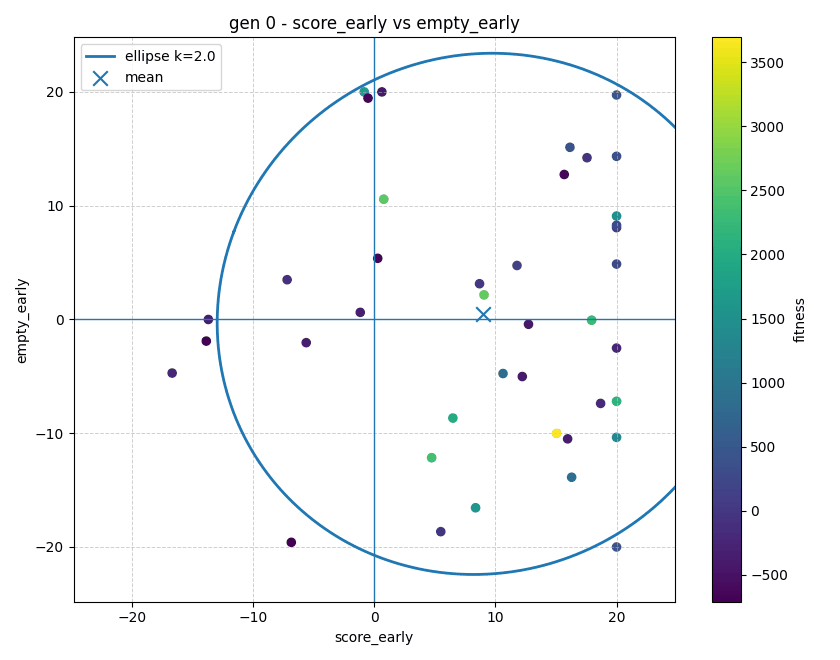
\includegraphics[width=0.75\linewidth]{first_frame.png}
    \caption{Début de l’apprentissage : exploration large de l’espace des poids.}
    \label{fig:cmaes_debut}
\end{figure}

\begin{figure}[H]
    \centering
    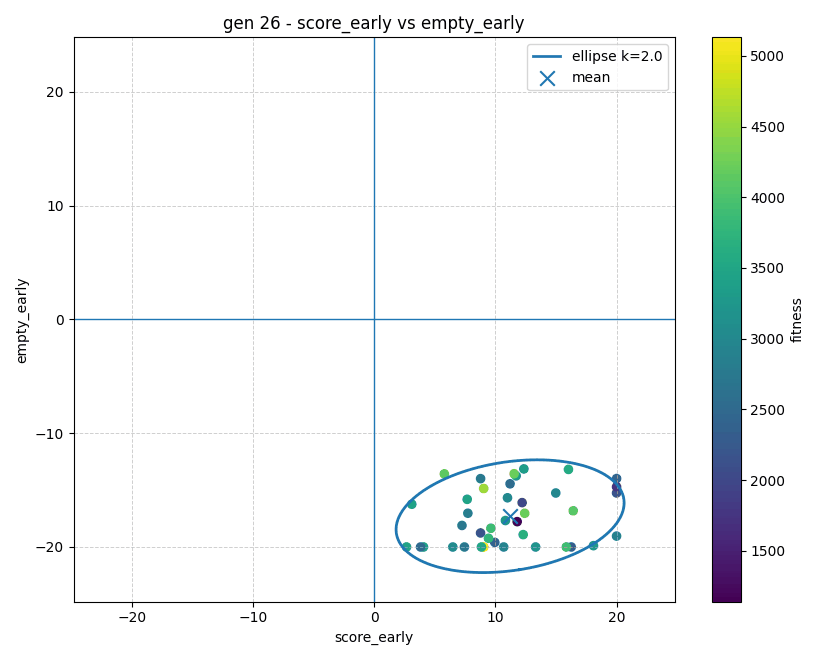
\includegraphics[width=0.75\linewidth]{last_frame.png}
    \caption{Fin de l’apprentissage : concentration des candidats autour de la moyenne optimisée.}
    \label{fig:cmaes_fin}
\end{figure}

\clearpage
\subsection{Évolution des poids (early / late)}
\label{annexe:C2}

La fonction d’évaluation utilise deux jeux de poids : un pour le début/milieu de partie (early) et un pour la fin de partie (late).  
Pendant l’apprentissage, les meilleurs poids sont sauvegardés à chaque itération.

À partir de ces données, je génère trois visualisations pour mieux analyser les valeurs apprises :

\begin{itemize}
    \item \textbf{Comparaison directe (early vs late)} : visualise, pour chaque heuristique, les deux poids et leur écart.
    \item \textbf{Différence $\Delta = w_{late} - w_{early}$} : montre quelles heuristiques sont davantage favorisées en fin ou en début de partie.
    \item \textbf{Interpolation au cours de la partie} : illustre la transition progressive entre les deux jeux de poids selon le coefficient de phase $\lambda$.
\end{itemize}

Les figures suivantes sont présentées ci-dessous. Elles illustrent ces données à titre d’exemple et ne correspondent pas à la configuration finale retenue.

\begin{figure}[H]
    \centering
    \includegraphics[width=0.8\linewidth]{images/weights_compare.png}
    \caption{Comparaison des poids early et late (points reliés) pour chaque heuristique.}
    \label{fig:poids_comparaison}
\end{figure}

\begin{figure}[H]
    \centering
    \includegraphics[width=0.8\linewidth]{images/weights_delta.png}
    \caption{Différence $\Delta = w_{late} - w_{early}$ : signe et amplitude de l’écart entre phases.}
    \label{fig:poids_delta}
\end{figure}

\begin{figure}[H]
    \centering
    \includegraphics[width=0.8\linewidth]{images/weights_over_phase.png}
    \caption{Interpolation des poids en fonction de la phase $\lambda$ (0 = late, 1 = early).}
    \label{fig:poids_interpolation}
\end{figure}

\section{Améliorations envisagées}
\label{annexe:ameliorations}

\begin{itemize}
    \item \textbf{History Heuristic :} testée mais non retenue, car elle diminuait légèrement les performances dans mon cas, malgré son usage fréquent dans les moteurs d’échecs.
    
    \item \textbf{Optimisation mémoire :} la table de transposition n’est jamais remplie à plus de 60\%, ce qui représente environ 20 MiB inutilisés ($\Rightarrow$ lui trouver une utilité).
    
    \item \textbf{Opening book :} idée de précalculer certaines ouvertures, abandonnée faute de temps d’apprentissage suffisant.
    
    \item \textbf{Base de fins de partie :} création d’un dataset d’endgames pour améliorer les positions finales critiques.
    
    \item \textbf{Table de transposition persistante :} remplissage d'une TT persistante pendant la phase d’apprentissage.
    
    \item \textbf{LMR plus avancé :} mise en place d’un système de réduction plus dynamique (type gestion par budget).
    
    \item \textbf{Heuristiques et poids :} ajout de nouvelles heuristiques et amélioration des poids actuels, probablement encore perfectibles.
\end{itemize}

\end{document}
